\documentclass{beamer}
\usetheme{Copenhagen}  %% Themenwahl
%% Language and font encodings
\usepackage[utf8x]{inputenc}
\usepackage[T1]{fontenc}
\usepackage[ngerman]{babel}

\title{Simulation eines Lichtstrahls nach Gitterdurchlauf}
\author{Simon Jung, Bernd Lienau, Alexander Franke}
\date{16. Januar 2018}





\usepackage{mathrsfs}
\usepackage[colorinlistoftodos]{todonotes}
%\usepackage[colorlinks=true, allcolors=blue]{hyperref}
%\newcommand{\ff}[1]{\mathscr{F}\left[#1\right]}




%\usepackage{ngerman}
%\usepackage[latin1]{inputenc}
%\usepackage[T1]{fontenc}
%\usepackage{german}
\usepackage{amssymb}
\usepackage{amsmath}
%\usepackage[utf8]{inputenc}
\usepackage{graphicx}
\usepackage{enumerate}
\usepackage{multirow}
\usepackage{subfigure}
\usepackage{dsfont}
\usepackage{slashed}
\usepackage{textcomp}
\usepackage{url}
\usepackage{hyperref}
\usepackage{float}
\usepackage{verbatim}
%\usepackage{underscore}

\setbeamertemplate{navigation symbols}{}

%_______________________________________________________________________________
\begin{document}


\begin{frame}
\maketitle
\end{frame}

%_______________________________________________________________________________

\begin{frame}
\begin{enumerate}
\item	Einleitung und Motivation
\item	Theoretische Grundlagen
	\begin{enumerate}
	\item	Skizzierung des Problems
	\item	Mathematische Beschreibung
	\item	Theoretisches Ergebnis
	\end{enumerate}
\item	Aufbau des Codes
	\begin{enumerate}
	\item	Flussdiagramm
	\item	Vorstellung der wichtigen Funktionen
	\item	Einbau der Fehler
	\end{enumerate}
\item	Simulierte Ergebnisse
	\begin{enumerate}
	\item	Ohne Fehler
	\item	mit Fehler
	\end{enumerate}
\end{enumerate}

\end{frame}


%_______________________________________________________________________________

\section{Theoretische Grundlagen}
\subsection{Skizzierung des Problems}
\begin{frame}
  \frametitle{Skizzierung des Einzelspalts}

%\begin{figure}[!htb]
%\centering
%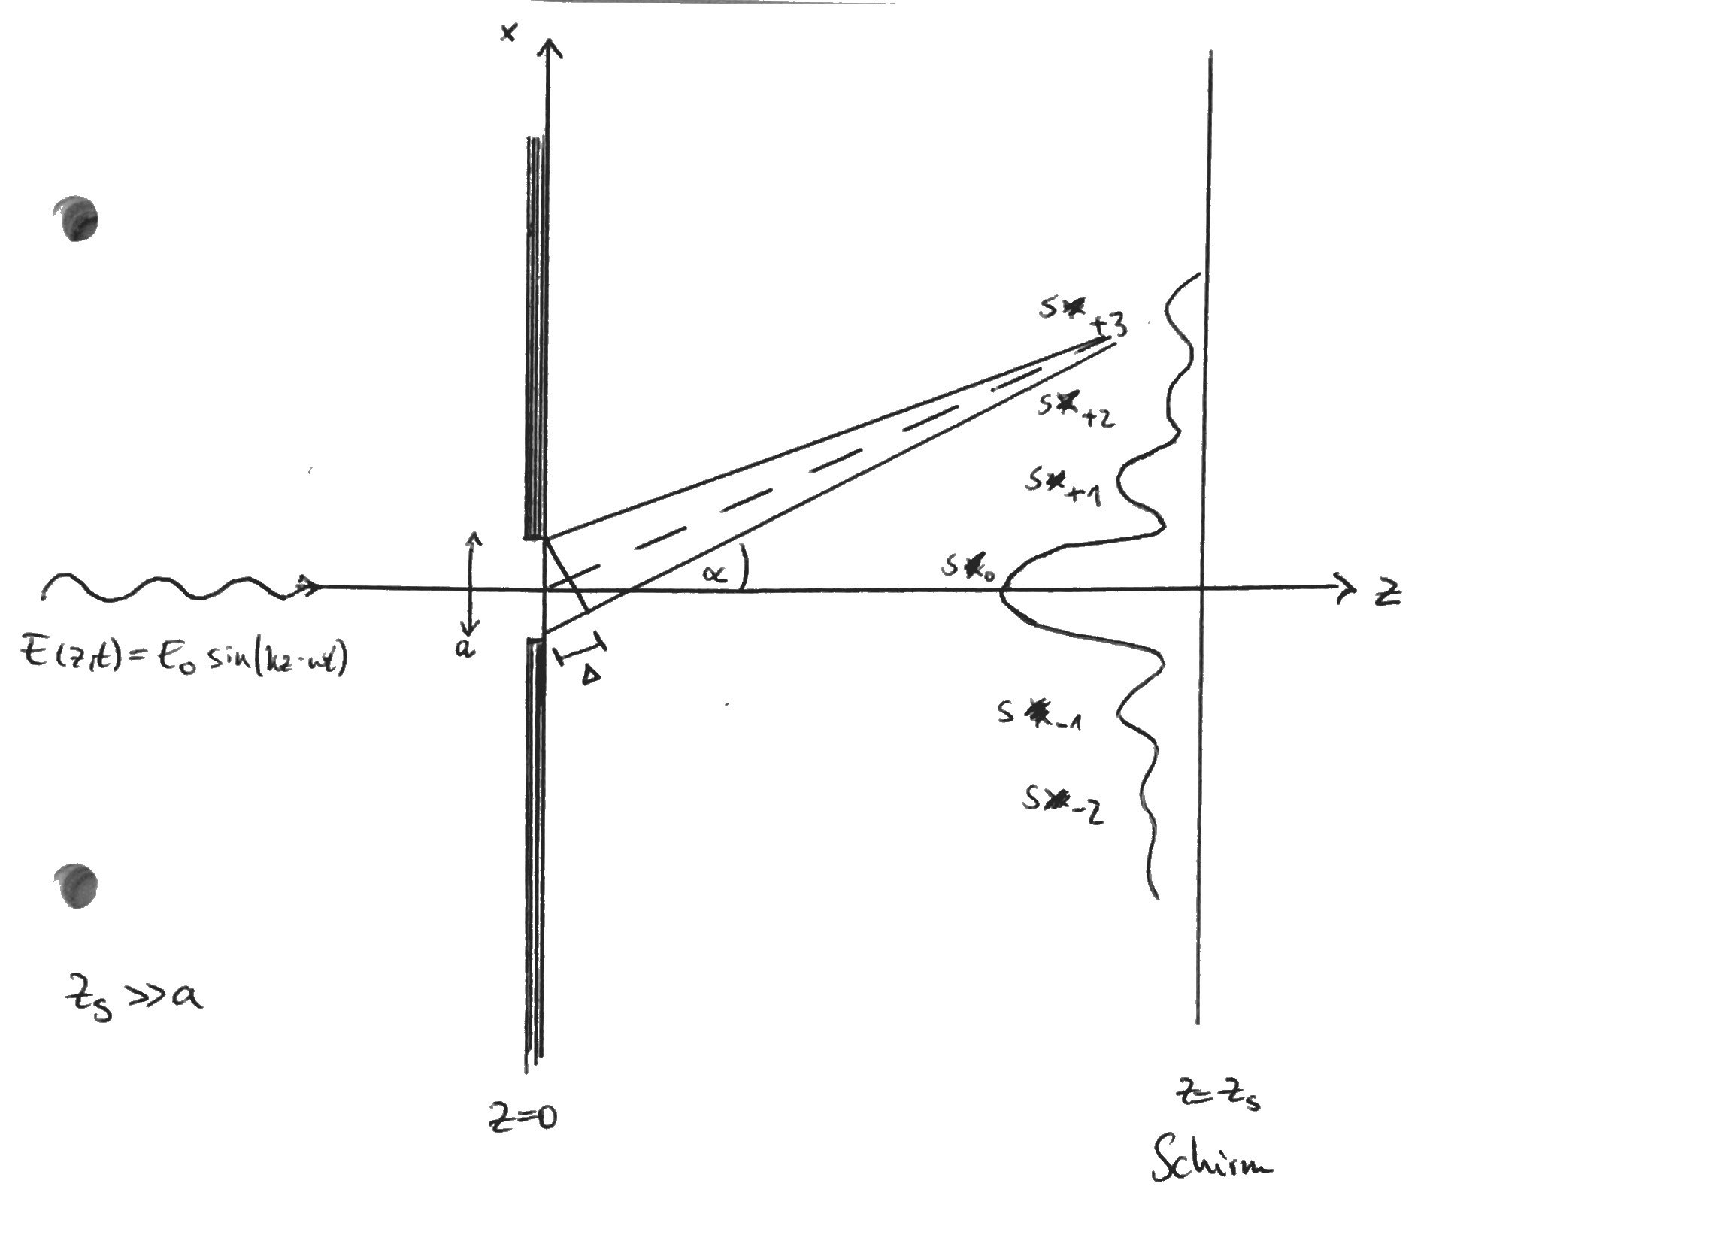
\includegraphics[width=\textwidth]{einzelspalt.pdf}
%\caption{Skizze mit allen relevanten Variablen für den Einzelspalt}
%\end{figure}
insert graph\\

\begin{align*}
I_S = I_0 \left( \frac{\sin\left(\frac{\pi a}{\lambda}\sin \alpha_x\right)}{\frac{\pi a}{\lambda} \sin \alpha_x} \right)^2
%\label{eq:einzelspalt_vorueberlegung}
\end{align*}





\end{frame}

%_______________________________________________________________________________

\begin{frame}
  \frametitle{Skizzierung des Doppelspalts}

%\begin{figure}[!htb]
%\centering
%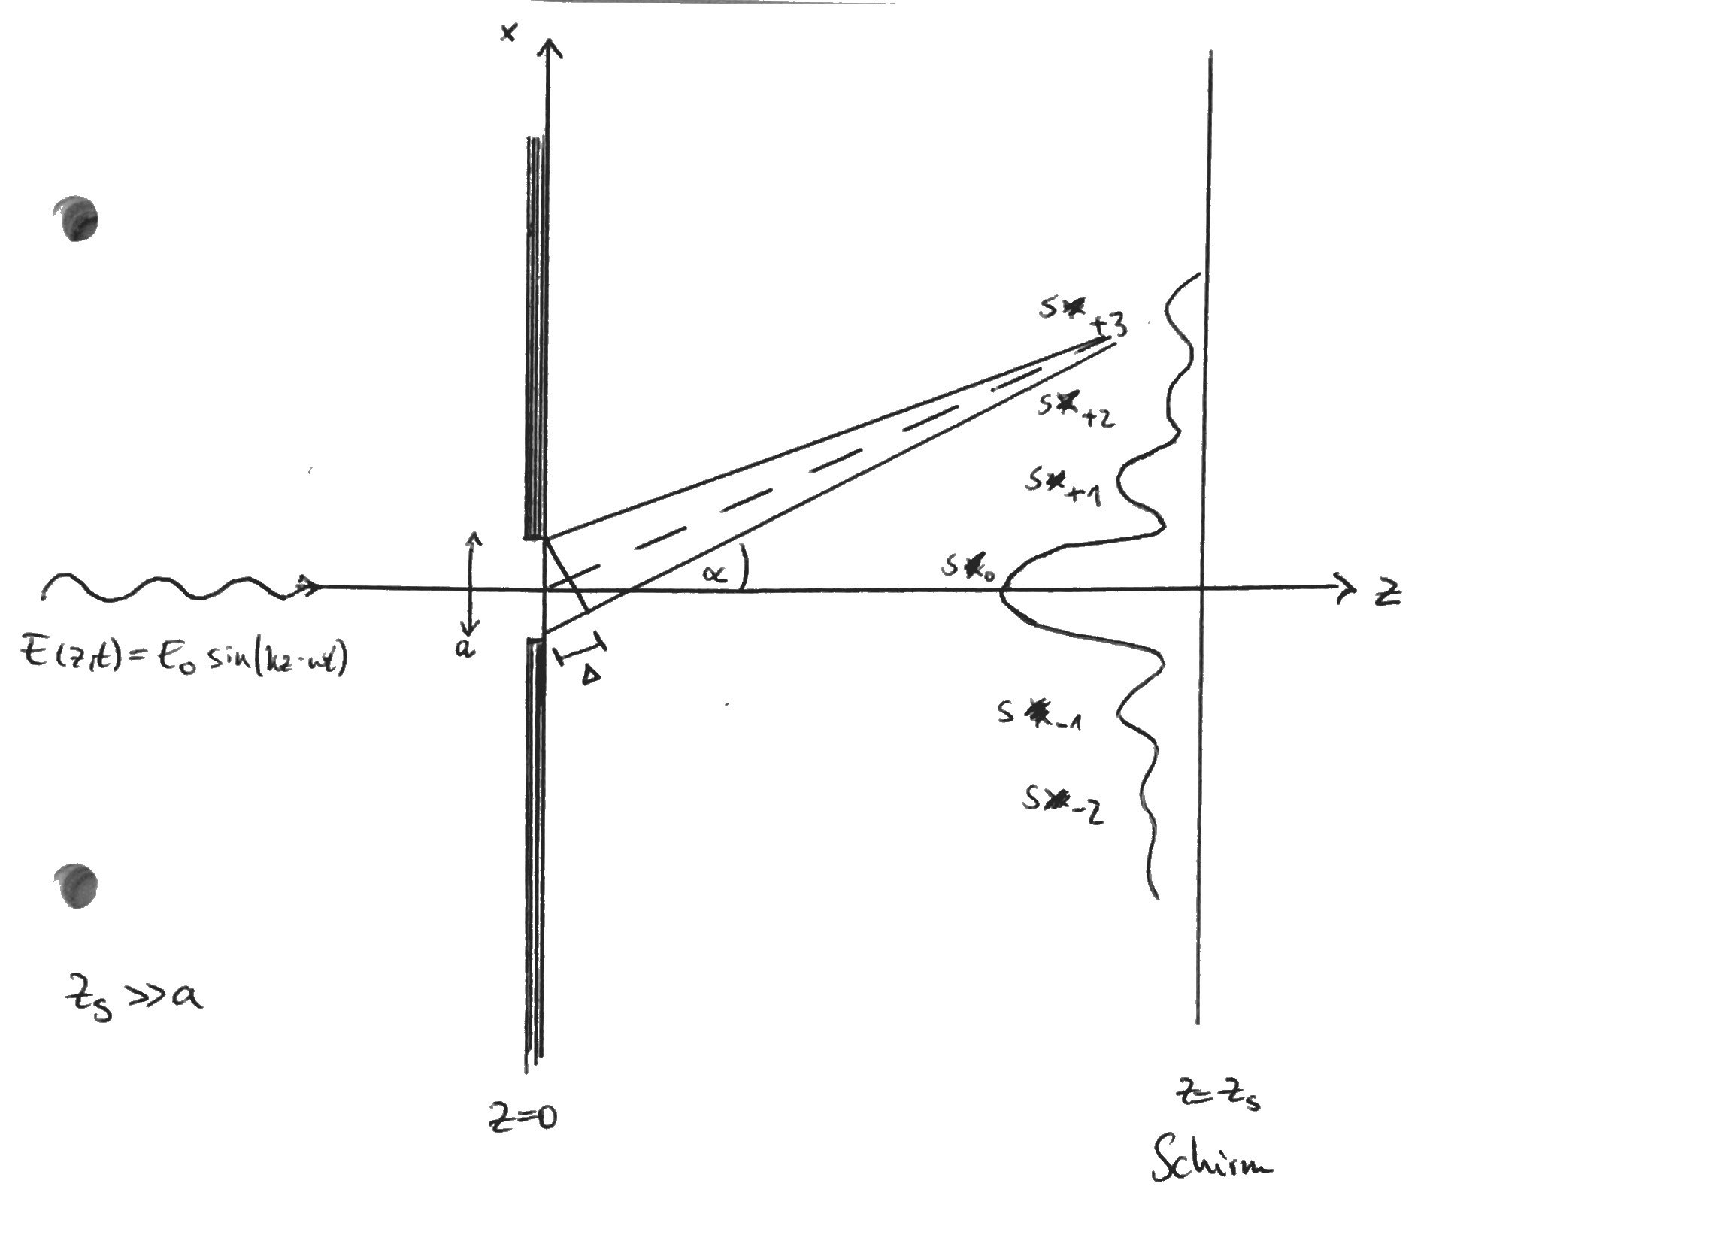
\includegraphics[width=\textwidth]{einzelspalt.pdf}
%\caption{Skizze mit allen relevanten Variablen für den Einzelspalt}
%\end{figure}
insert graph\\

\begin{align*}
I(\alpha_x,0) = |\Psi(\alpha_x,0)|^2 =  \cos^2 \left(\frac{\pi d \sin(\alpha_x)}{\lambda}\right) \frac{\sin^2(\pi a \sin(\alpha_x)/\lambda)}{(\pi a \sin(\alpha)/\lambda)^2}
\end{align*}


\end{frame}


%_______________________________________________________________________________

\subsection{Mathematische Beschreibung}
\begin{frame}
  \frametitle{Mathematische Beschreibung}

Allgemein ist die Wellenfunktion des Beugungsbildes gegeben durch

\begin{align*}
\Psi (u,v) = \int \int f(x,y) \exp\Big(-i(ux+vy)\Big) dx dy
\end{align*}
wobei $u= k_0 \sin\alpha_x$ und $v=k_0\sin\alpha_y$




\end{frame}


%_______________________________________________________________________________

\begin{frame}
  \frametitle{Mathematische Beschreibung}

Einzelspalt:
\begin{align*}
f_\text{ES}(x) = \begin{cases} 
1  &\text{für } |x| <  \frac{a}{2} \\
0 & \text{sonst}\end{cases}
\label{eq:einzelspalt}
\end{align*}

Ein kleines rechteckiges Loch der Höhe $h$ und Breite $a$:
\begin{align*}
\Psi(\alpha_x,\alpha_y) &= g(x) \cdot h(y) \\
&= \int_{-a/2}^{a/2} e^{-ixk\sin(\alpha_x)} dx \int_{-h/2}^{h/2} e^{-iyk\sin(\alpha_y)}dy\\
&= ah \frac{\sin(\frac{1}{2} ak\sin(\alpha_x))}{\frac{1}{2} ak\sin(\alpha_x)} \cdot \frac{\sin(\frac{1}{2} hk\sin(\alpha_y))}{\frac{1}{2} hk\sin(\alpha_y)}\\
\end{align*}

\begin{align*}
\Psi (\xi,\phi ) = \pi R^2 \left( \frac{2J_1(\xi R)}{\xi R} \right)
\end{align*}
mit 
\begin{align*}
J_{1}(x)=\sum _{{r=0}}^{\infty }{\frac  {(-1)^{r}({\frac  {x}{2}})^{{2r+1 }}}{\Gamma (1 +r+1)r!}}\, 
\end{align*}



\end{frame}



%_______________________________________________________________________________

\begin{frame}
  \frametitle{Doppelspalt}

\begin{block}
Aufgrund der Eigenschaften der Fouriertransformierten, können wir die Überlagerung von Beugungsmustern als algebrische Summe der Transmissionsfunktion einfacher Objekte aufschreiben. Im Allgemeinen muss bei der Transformierten des Gesamtobjektes, Real- und Imaginärteil getrennt addiert werden. Nur für den Sonderfall von Punktsymmetrie bezüglich der Mitte sind die Transformierten reell. 
\end{block}

\begin{block}
Wir betrachten nun die Überlagerung der beiden Beugungsmuster der Einzelspalte. Die Eigenschaften der Fouriertransformation machen dieses Vorgehen sehr viel einfacher, da wir wissen, dass
\begin{align*}
g(x) \circledast h(y) = \mathscr{F}[g(x)] \cdot \mathscr{F}[h(y)] \\
\end{align*}
\end{block}

\end{frame}


%_______________________________________________________________________________

\begin{frame}
  \frametitle{Viele-Spalte}

Ähnlich wie beim Doppelspalt brauchen wir eine Faltung von einer Transmissionsfunktions des Gitters mit der des Einzelspaltes.
\begin{align*}
f_\text{Gitter} \circledast f_\text{ES} = \left[\sum_{n=-N/2}^{N/2} \delta\left(x-nd\right)\right]  \circledast f_\text{ES}
\end{align*}
Die Fouriertransformation wird zu 
\begin{align*}
\Psi(\alpha_x) = \left[\sum_{m=-N/2}^{N/2}\exp\Big(-ik\sin(\alpha_x)md\Big)\right]  \circledast f_\text{ES} = \left[\sum_{m=-N/2}^{N/2}\exp\Big(-ik\sin(\alpha_x)d\Big)^m\right]  \circledast f_\text{ES}
\end{align*}

\end{frame}


%_______________________________________________________________________________

\begin{frame}
  \frametitle{Viele-Spalte 2}

Lassen wir nun N gegen unendlich laufen haben wir 
\begin{align*}
\Psi(\alpha_x) = \sum_{m=-\infty}^\infty \delta \left((k\sin\alpha_x - \frac{2\pi m}{d}\right)
\end{align*}

Für endliches N erhalten wir mit der geometrischen Reihe
\begin{align*}
	\Psi(\alpha_x) = \frac{1- \exp(-ik \sin(\alpha_x)Nd)}{1-\exp(-ik\sin(\alpha_x)d)}
\end{align*}
Damit erhalten wir folgende Intensität
\begin{align*}
I_\text{Gitter} = |\Psi(\alpha_x)|^2 = \frac{\sin^2(Nk\sin(\alpha_k) d /2)}{\sin^2(k\sin(\alpha_k) d /2)}
\end{align*}

\end{frame}



%_______________________________________________________________________________

\section{Aufbau des Codes}
\subsection{Flussdiagramm}
\begin{frame}
  \frametitle{Flussdiagramm}

%\begin{figure}[!htb]
%\centering
%\includegraphics[width=\textwidth]{?}
%\caption{Flussdiagramm}
%\end{figure}
insert graph\\







\end{frame}





%_______________________________________________________________________________

\subsection{Vorstellung der wichtigen Funktionen}
\begin{frame}
  \frametitle{Wichtige Funktionen}







\end{frame}


%_______________________________________________________________________________

\begin{frame}
  \frametitle{Wichtige Funktionen}







\end{frame}


%_______________________________________________________________________________

\section{Simulierte Ergebnisse}
\subsection{Ohne Fehler}
\begin{frame}
  \frametitle{Einzelspalte}

%\begin{figure}[!htb]
%\centering
%\includegraphics[width=\textwidth]{?}
%\caption{Einzelspalte}
%\end{figure}
insert graph\\

\end{frame}

%_______________________________________________________________________________

\begin{frame}
  \frametitle{Doppelspalt}

%\begin{figure}[!htb]
%\centering
%\includegraphics[width=\textwidth]{?}
%\caption{Doppelspalt}
%\end{figure}
insert graph\\

\end{frame}


%_______________________________________________________________________________

\begin{frame}
  \frametitle{Mehrfachspalte}

%\begin{figure}[!htb]
%\centering
%\includegraphics[width=\textwidth]{?}
%\caption{Mehrfachspalte}
%\end{figure}
insert graph\\

\end{frame}


%_______________________________________________________________________________

\subsection{Mit Fehler}
\begin{frame}
  \frametitle{Mehrfachspalt mit Fehler}

%\begin{figure}[!htb]
%\centering
%\includegraphics[width=\textwidth]{?}
%\caption{Mehrfachspalt mit Fehler}
%\end{figure}
insert graph\\


\end{frame}













\end{document}